\providecommand{\main}{../..}
\documentclass[\main/thesis.tex]{subfiles}
\begin{document}

\section{Incrementing a Numeral}\label{increment}

Given a numeral \lstinline|xs| of \lstinline|Numeral b d o|
and a proof of \lstinline|¬ (Maximum xs)|,
with functions and theorems constructed in the last section, we can:

\begin{itemize}
    \item Find the next numeral of \lstinline|xs| using \lstinline|next-numeral|.
    \item Know that the next numeral will be greater than \lstinline|xs|
        by \lstinline|next-numeral-is-greater|.
    \item Know that the next numeral will be the least numeral that is greater
        than \lstinline|xs| by \lstinline|next-numeral-is-immediate|.
\end{itemize}

However, none of the theorems above guarantees that the next numeral will be the
\textbf{successor} of \lstinline|xs|, i.e., the next numeral and \lstinline|xs|
differs by only $ 1 $.
For example, we have seen from the previous section that numerals of
\lstinline|GappedEndpoint| of systems of \lstinline|Proper| have no successors.

\begin{center}
    \begin{adjustbox}{max width=\textwidth}
        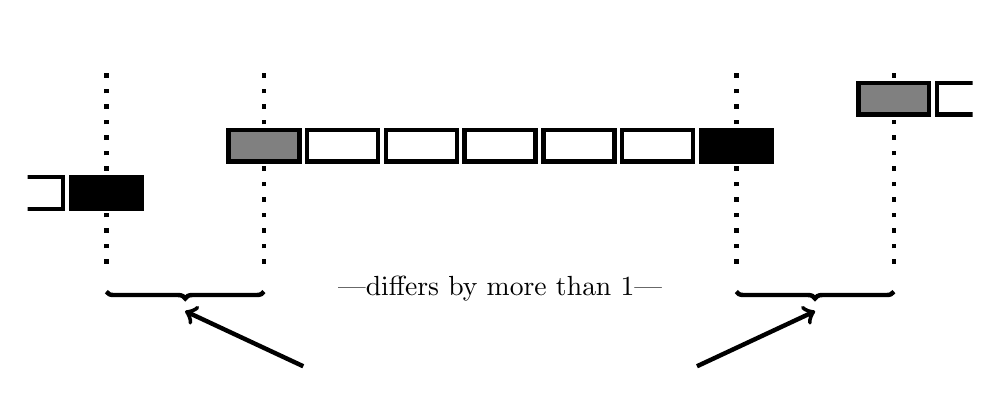
\begin{tikzpicture}
            % the frame
            \path[clip] (5.5, -3) rectangle (17.5, 1.5);


            % ticks
            \draw[ultra thick, loosely dotted] (6.5,-1.5) -- (6.5,1);
            \draw[ultra thick, loosely dotted] (8.5,-1.5) -- (8.5,1);
            \draw[ultra thick, loosely dotted] (14.5,-1.5) -- (14.5,1);
            \draw[ultra thick, loosely dotted] (16.5,-1.5) -- (16.5,1);

            \draw[ultra thick, decoration={brace,mirror,raise=10},decorate]
                (6.5,-1.5) -- (8.5,-1.5);
            \draw[ultra thick, decoration={brace,mirror,raise=10},decorate]
                (14.5,-1.5) -- (16.5,-1.5);
            \node[below=1] at (11.5, -1.5) {\lstinline|differs by more than 1|};

            % the body
            \foreach \i in {0,...,2} {
                \draw[ultra thick, fill=gray] ({\i*8+0.05}, {\i*0.6-0.8}) rectangle ({\i*8+0.95}, {\i*0.6-0.4});
                \foreach \j in {1,...,5} {
                    \draw[ultra thick] ({\i*8+\j+0.05}, {\i*0.6-0.8}) rectangle ({\i*8+\j+0.95}, {\i*0.6-0.4});
                };
                \draw[ultra thick, fill=black] ({\i*8+6.05}, {\i*0.6-0.8}) rectangle ({\i*8+6.95}, {\i*0.6-0.4});
            };

            \coordinate (A) at (7.5, -2.1);
            \coordinate (B) at (9, -2.8);
            \coordinate (C) at (15.5, -2.1);
            \coordinate (D) at (14, -2.8);

            \path[->, ultra thick] (B) edge node {} (A);
            \path[->, ultra thick] (D) edge node {} (C);

        \end{tikzpicture}
    \end{adjustbox}
\end{center}

Suppose we are to define a function called \lstinline|increment| that returns
the successor of a given numeral.
For those numerals that are eligible for increment,
we can simply compute them with \lstinline|next-numeral|;
and for those that are not eligible, we need a predicate for discriminating them.

\subsubsection{\lstinline|Incrementable|}

Similar to the definition of \lstinline|Bounded|, we define the predicate
\lstinline|Incrementable| as an existential proposition.
To prove that a numeral \lstinline|xs| is \lstinline|Incrementable|,
one is oblidged to present the successor \textit{and} a proof to justify it.

\begin{lstlisting}[basicstyle=\ttfamily\scriptsize]
Incrementable : ∀ {b d o} → (xs : Numeral b d o) → Set
Incrementable {b} {d} {o} xs = Σ[ xs' ∈ Numeral b d o ] ⟦ xs' ⟧ ≡ suc ⟦ xs ⟧
\end{lstlisting}

We can then develop theorems about \lstinline|Incrementable|.

\subsubsection{Excluding Maximum Numerals}

If a numeral is a maximum, then there is no such a thing as the next numeral,
much less a successor.

\begin{lstlisting}
Maximum⇒¬Incrementable : ∀ {b d o}
    → (xs : Numeral b d o)
    → (max : Maximum xs)
    → ¬ (Incrementable xs)
Maximum⇒¬Incrementable xs max (incremented , claim)
    = contradiction
        (max incremented)
        (>⇒≰ (m≡1+n⇒m>n claim))
%
\end{lstlisting}
where \lstinline|incremented| is the claimed successor
and \lstinline|claim : ⟦ incremented ⟧ ≡ suc ⟦ xs ⟧|.
This is proven by contradicting these two propositions:

\begin{itemize}
    \item \lstinline|max incremented : ⟦ xs ⟧ ≥ ⟦ incremented ⟧|
    \item \lstinline|>⇒≰ (m≡1+n⇒m>n claim) : ⟦ xs ⟧ ≰ ⟦ incremented ⟧|
\end{itemize}

\subsubsection{Excluding Numerals at Gapped Endpoints}

The next kind of numerals to be excluded is the ones that are located at gapped
endpoints.

\begin{center}
    \begin{adjustbox}{max width=\textwidth}
        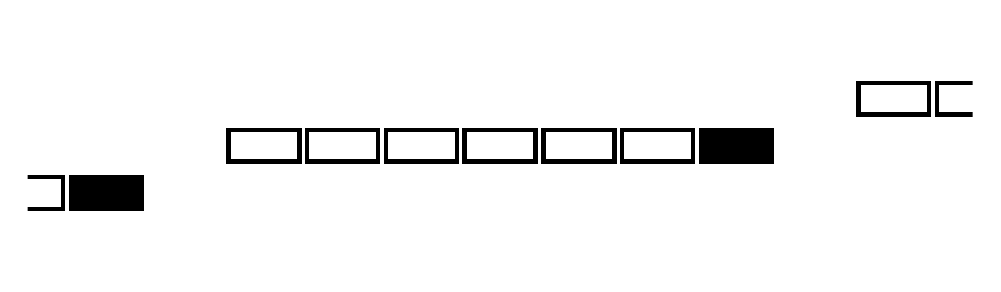
\begin{tikzpicture}
            % the frame
            \path[clip] (5.5, -1.5) rectangle (17.5, 1.5);

            % the body
            \foreach \i in {0,...,2} {
                \foreach \j in {0,...,5} {
                    \draw[ultra thick] ({\i*8+\j+0.05}, {\i*0.6-0.8}) rectangle ({\i*8+\j+0.95}, {\i*0.6-0.4});
                };
                \draw[ultra thick, fill=black] ({\i*8+6.05}, {\i*0.6-0.8}) rectangle ({\i*8+6.95}, {\i*0.6-0.4});
            };
        \end{tikzpicture}
    \end{adjustbox}
\end{center}

\begin{lstlisting}[basicstyle=\ttfamily\scriptsize]
GappedEndpoint⇒¬Incrementable : ∀ {b d o}
    → (xs : Numeral (suc b) (suc d) o)
    → (greatest : Greatest (lsd xs))
    → (proper : 2 ≤ suc (d + o))
    → (gapped : Gapped xs proper)
    → ¬ (Incrementable xs)
GappedEndpoint⇒¬Incrementable xs greatest proper gapped (incremented , claim)
    = contradiction ⟦next⟧>⟦incremented⟧ ⟦next⟧≯⟦incremented⟧
\end{lstlisting}

This is also proven by contradicting two propositions.

First, we show that the next numeral is greater than the claimed successor
by rephrasing the lemma \lstinline|next-numeral-Proper-GappedEndpoint-lemma|.
As a side note, \lstinline|next-numeral-Proper| delegates tasks to other helper
functions. \lstinline|next-numeral-Proper-refine| is here to narrow the term
computed by \lstinline|next-numeral-Proper| down to
\lstinline|next-numeral-Proper-GappedEndpoint|
by giving evidences that it is delegated that way.

\begin{lstlisting}[basicstyle=\ttfamily\scriptsize]
⟦next⟧>⟦incremented⟧ : ⟦ next-numeral-Proper xs proper ⟧ > ⟦ incremented ⟧
⟦next⟧>⟦incremented⟧ =
    start
        suc ⟦ incremented ⟧
    ≈⟨ cong suc claim ⟩
        suc (suc ⟦ xs ⟧)
    ≤⟨ next-numeral-Proper-GappedEndpoint-lemma xs greatest proper gapped ⟩
        ⟦ next-numeral-Proper-GappedEndpoint xs proper gapped ⟧
    ≈⟨ cong ⟦_⟧ (sym (next-numeral-Proper-refine
        xs proper (GappedEndpoint b d o greatest gapped)))
    ⟩
        ⟦ next-numeral-Proper xs proper ⟧
    □
\end{lstlisting}

However, the next numeral should only be greater than the given numeral
\lstinline|xs| and nothing else.

\begin{lstlisting}[basicstyle=\ttfamily\scriptsize]
⟦next⟧≯⟦incremented⟧ : ⟦ next-numeral-Proper xs proper ⟧ ≯ ⟦ incremented ⟧
⟦next⟧≯⟦incremented⟧ = ≤⇒≯ (next-numeral-is-immediate-Proper
    xs incremented proper (m≡1+n⇒m>n claim))
\end{lstlisting}

\subsubsection{Deciding Incrementable Numerals}

Together with lemmata about other kinds of numerals:

\begin{itemize}
    \item \lstinline|next-numeral-Proper-Interval-lemma|
    \item \lstinline|next-numeral-Proper-UngappedEndpoint-lemma|
\end{itemize}

We can decide if a numeral of \lstinline|Proper| is incrementable.

\begin{lstlisting}[basicstyle=\ttfamily\scriptsize]
Incrementable?-Proper : ∀ {b d o}
    → (xs : Numeral (suc b) (suc d) o)
    → (proper : 2 ≤ suc (d + o))
    → Dec (Incrementable xs)
Incrementable?-Proper xs proper with nextView xs proper
Incrementable?-Proper xs proper | Interval b d o ¬greatest
    = yes ((next-numeral-Proper xs proper) , (begin
            ⟦ next-numeral-Proper xs proper ⟧
        ≡⟨ cong ⟦_⟧ (next-numeral-Proper-refine xs proper
            (Interval b d o ¬greatest))
        ⟩
            ⟦ next-numeral-Proper-Interval xs ¬greatest proper ⟧
        ≡⟨ next-numeral-Proper-Interval-lemma xs ¬greatest proper ⟩
            suc ⟦ xs ⟧
        ∎))
Incrementable?-Proper xs proper | GappedEndpoint b d o greatest gapped
    = no (GappedEndpoint⇒¬Incrementable xs greatest proper gapped)
Incrementable?-Proper xs proper | UngappedEndpoint b d o greatest ¬gapped
    = yes ((next-numeral-Proper xs proper) , (begin
            ⟦ next-numeral-Proper xs proper ⟧
        ≡⟨ cong ⟦_⟧ (next-numeral-Proper-refine xs proper
            (UngappedEndpoint b d o greatest ¬gapped))
        ⟩
            ⟦ next-numeral-Proper-UngappedEndpoint xs greatest proper ¬gapped ⟧
        ≡⟨ next-numeral-Proper-UngappedEndpoint-lemma xs greatest proper ¬gapped ⟩
            suc ⟦ xs ⟧
        ∎))
\end{lstlisting}

\paragraph{Summary of numerals of \lstinline|Proper|}

\begin{center}
    \begin{adjustbox}{max width=\textwidth}
    \begin{tabular}{ | l | c | c | c | }
    \textbf{Property} & \textbf{Interval} & \textbf{GappedEndpoint} & \textbf{UngappedEndpoint} \\
    \hline
    is incrementable     & yes & no & yes  \\
    \end{tabular}
    \end{adjustbox}
\end{center}

Putting everything together, we can also determine numerals of other categories.

\begin{lstlisting}
Incrementable? : ∀ {b d o}
    → (xs : Numeral b d o)
    → Dec (Incrementable xs)
Incrementable? xs with Maximum? xs
Incrementable? xs | yes max = no (Maximum⇒¬Incrementable xs max)
Incrementable? {b} {d} {o} xs | no ¬max with numView b d o
Incrementable? xs | no ¬max | NullBase d o
    = yes ((next-numeral-NullBase xs ¬max) ,
        (next-numeral-NullBase-lemma xs ¬max))
Incrementable? xs | no ¬max | NoDigits b o
    = no (NoDigits-explode xs)
Incrementable? xs | no ¬max | AllZeros b
    = no (contradiction (Maximum-AllZeros xs) ¬max)
Incrementable? xs | no ¬max | Proper b d o proper
    = Incrementable?-Proper xs proper
\end{lstlisting}

\paragraph{Summary}

\begin{center}
    \begin{adjustbox}{max width=\textwidth}
    \begin{tabular}{|l|c|c|c|c|c|c|}
        \hline
        \multirow{2}{*}{\textbf{Properties}} &
        \multirow{2}{*}{\textbf{NullBase}} &
        \multirow{2}{*}{\textbf{NoDigits}} &
        \multirow{2}{*}{\textbf{AllZeros}} &
        \multicolumn{3}{c|}{\textbf{Proper}} \\
        \cline{5 - 7}
        & & & & \textbf{Inteval} & \textbf{Gapped} & \textbf{Ungapped} \\
        \hline
        has an maximum     & yes & no & yes & no & no & no \\
        has an upper bound & yes & no & yes & no & no & no \\
        can be incremented
        \footnote{In case that the given numeral is not a maximum.}
         & yes & no & no  & yes & no & yes \\
        \hline
    \end{tabular}

    %
    % \begin{tabular}{ | l | c | c | c | c | c | c |}
    % \hline
    % \multirow{2}{*}{\textbf{Properties}} &
    % \multirow{2}{*}{\textbf{NullBase}} &
    % \multirow{2}{*}{\textbf{NoDigits}} &
    % \multirow{2}{*}{\textbf{AllZeros}} &
    % \multicolumn{3}{c|}{\textbf{Proper}} \\
    % % %
    % % \cline{5-7} & \textbf{Interval} & \textbf{GappedEndpoint} & \textbf{UngappedEndpoint} & fuck \\
    % % \hline
    % % is incrementable     & yes & no & yes & yes & no & yes \\
    % \end{tabular}
    \end{adjustbox}
\end{center}


\end{document}
